\problemname{Jabbing Jets}

\illustration{0.19}{showerhead.jpg}{CC BY 3.0 by gratuit on freeimageslive.co.uk\\\vspace{-4em}}
% Source: URL to image.

% optionally define variables/limits for this problem
\newcommand{\showermaxn}{10^4}
\newcommand{\showermaxdist}{10^4}

You have just gotten a new job at the Bathroom Accessories Production Company.
The first task you are given is to jab holes into showerheads.
To prove yourself, you have decided you want to create as many holes as possible.

However, you cannot just randomly drill holes everywhere in the showerhead.\footnote{At least, not without getting fired.}
In order to ensure that the showerheads look aesthetically pleasing,
the company has composed some guidelines which you will have to follow. See Figure \ref{fig:J-example} for some examples of aesthetically pleasing showerheads.
\begin{itemize}
\item The holes should be arranged in concentric circles of radii $r_1, r_2, \ldots, r_n$:
    the center of every hole should be on one of these circles.
\item \mbox{The distance between the centers of any two holes should be at least $e$.}
\end{itemize}

How many holes can you make at most?

\begin{figure}[htb]
	\centering
	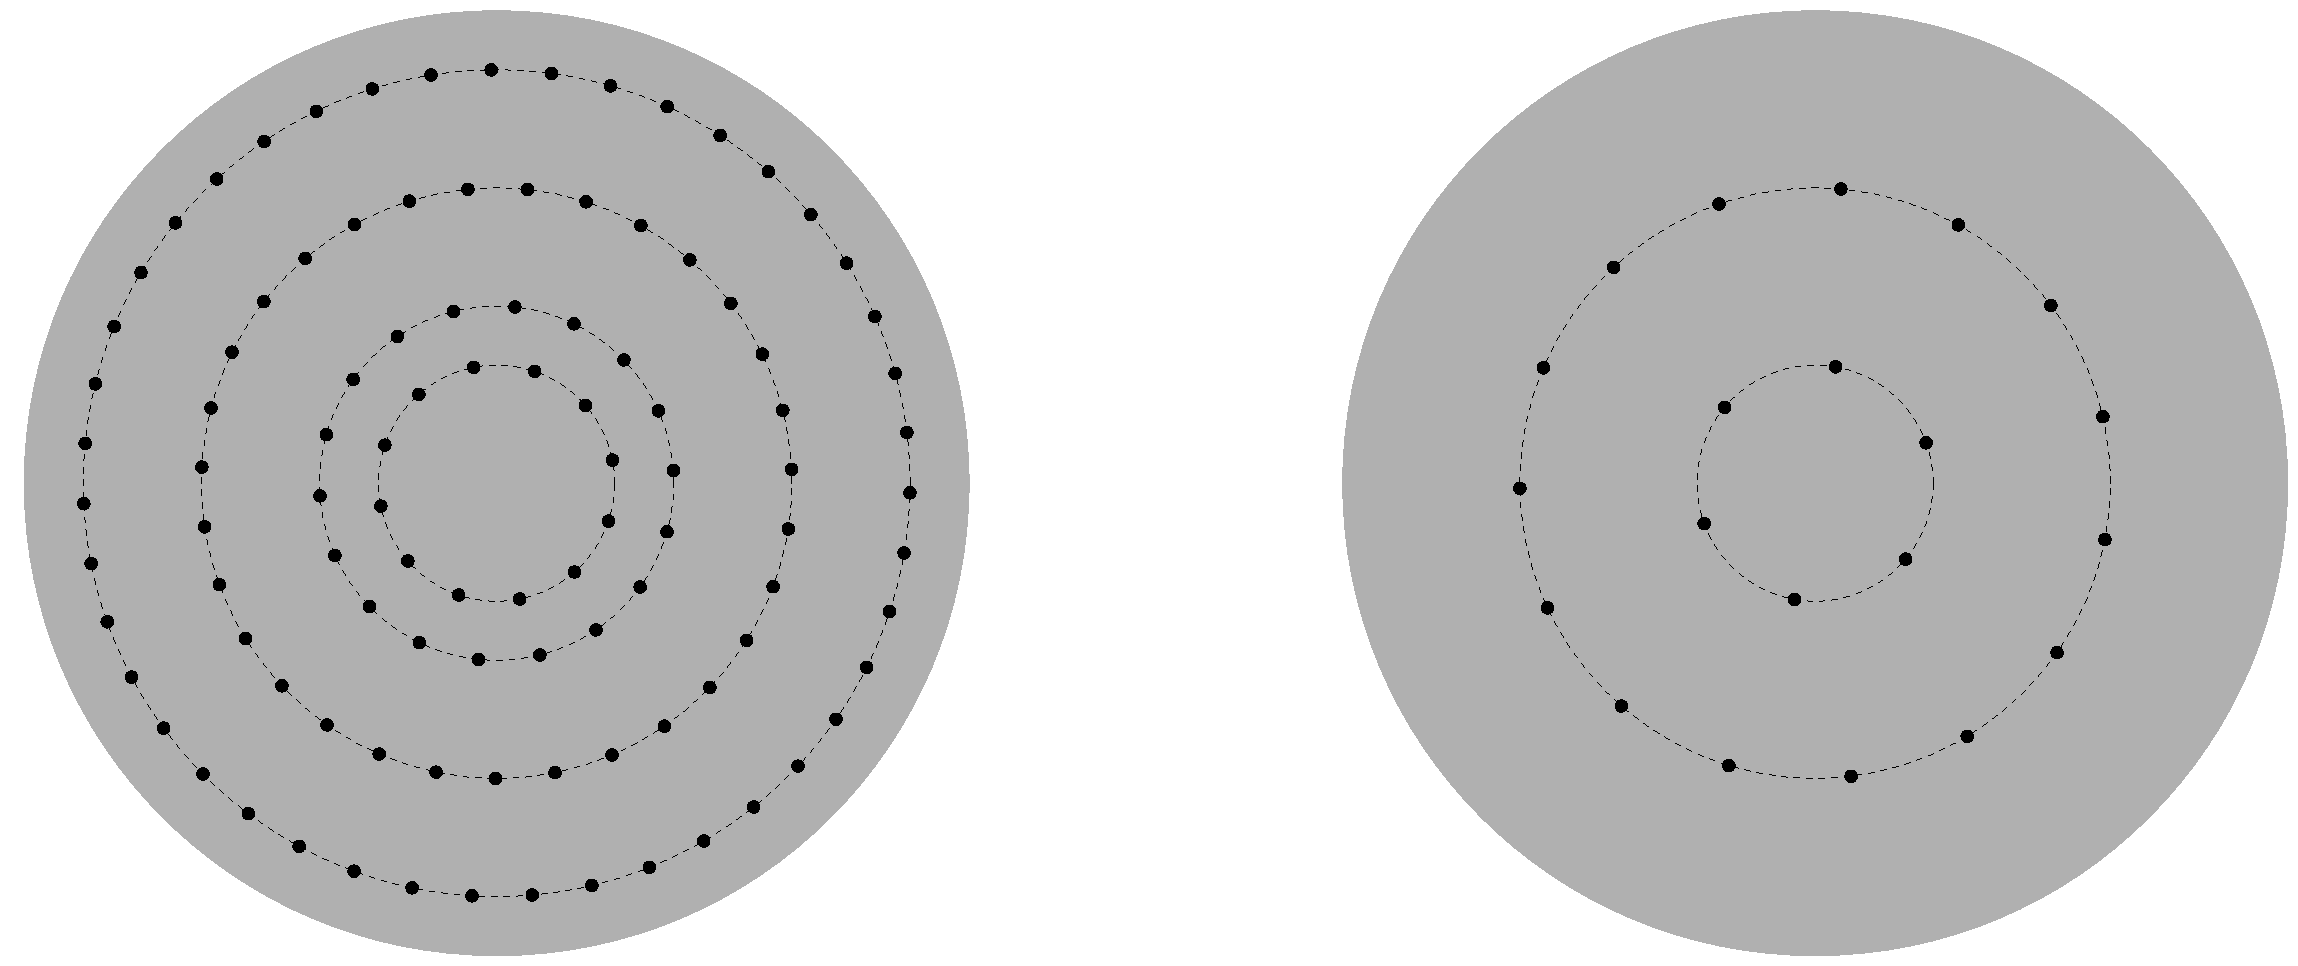
\includegraphics[width=0.7\textwidth]{figure.pdf}
	\caption{
		Possible aesthetically pleasing showerheads for the first two samples.
	}
	\label{fig:J-example}
\end{figure}

\begin{Input}
    The input consists of:
    \begin{itemize}
        \item One line with two integers $n$ and $e$
			($1 \leq n, e \leq \showermaxn$), % = \showermaxdist
			the number of circles and the minimal distance between holes.
		\item One line with $n$ integers $r_1, \ldots, r_n$
			($1 \leq r_i \leq \showermaxdist$), the radii of the circles.
    \end{itemize}
    It is guaranteed that the numbers $r_i$ are given in increasing order, and
    that $r_{i+1} - r_i \geq e$.
    Furthermore, it is guaranteed that increasing any radius $r_i$ by at most $10^{-6}$
    will not change the final answer.
\end{Input}

\begin{Output}
    Output the maximal number of holes that you can make in the showerhead.
\end{Output}
